\section{Theorie}
\label{sec:Theorie}

%Gleichungen die dringend in der Auswertung benötigt werden:

%E=hc/\lambda              \label{eqn:E=hc/lambda}
%vgl. Versuchsanleitung    \label{eqn:(3)}
%vgl. Versuchsanleitung    \label{eqn:(4)}
%T=I_Al/I_0                \label{eqn:trans}
%\lambda = \frac{T-b}{a}   \label{eqn:lambda}  was auch immer a und b dann bei dir sind. aber für die Auswertung ist die echt essenziell

%du kannst die Label gerne umbenennen, ich habe sie jetzt nur erstmal in der Auswertung so genannt. Wenn du die Umbenennst, sag einfach bescheid. :)
\subsection{Die Änderung der Wellenlänge}
Wenn $\gamma$ -Strahlung an einem Elektron gestreut wird, beobachtet man eine Verschiebung der Wellenlänge hin zu längeren Wellenlängen.
Dies bezeichnet man als Compton-Effekt.
Wenn Röntgenstrahlung an Materie gestreut wird, wechselwirkt das Röntgenquant (das Photon) mit einem freien Elektron.
Dabei findet sowohl die kohärente Streuung als auch die inkohärente Streuung statt. Hierbei bezeichnet die kohärente Streuung
die klassische inelastische Streuung und die inkohärente die elastische, frequenzverschobene Streuung.
Die inelastische oder kohärente Streuung wird auch als Compton-Streuung bezeichnet.
Bei dieser gibt das Röntgenquant einen Teil seiner Energie an das Elektron ab. Dabei wird das Röntgenquant in einem Winkel $\theta$
gestreut. Da die Quantenenergie des Röntgenquants durch
\begin{equation}
	\label{eqn:E=hc/lambda}
	E =  \frac{h c}{\lambda}
\end{equation}
beschrieben wird, kommt es durch die Energieabgabe an das Elektron zu einer Verlängerung der Wellenlänge des Röntgenquants.
Für die Veränderung der Wellenlänge des Photons gilt
\begin{equation}
	\label{eqn:deltalambda}
	\increment \lambda = \frac{h}{m_e c} (1- \cos  \theta).
\end{equation}
Hierbei bezeichnet $\theta$ den Winkel zwischen einfallendem Photon und gestreutem Photon. Dies ist in Abbildung \ref{fig:StreuungPhoton}
dargestellt.
\begin{figure}[H]
	\centering
	\label{fig:StreuungPhoton}
	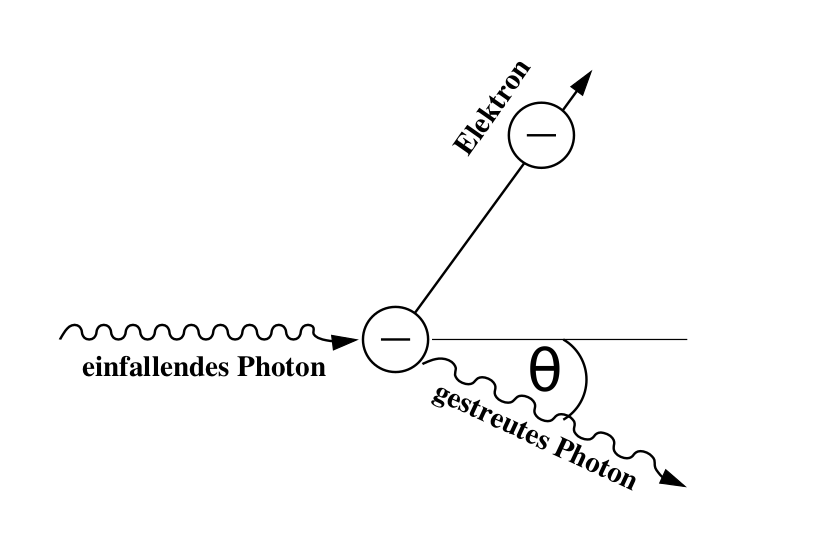
\includegraphics[scale=0.3]{content/comptoneffekt.png}
\end{figure}
\noindent
Daher ist die Verschiebung dann minimal, wenn $\theta = 0 \si{\degree}$ und maximal, wenn $\theta = 180 \si{\degree}$ ist.
Hierbei wird der Term $\lambda_c = \frac{h}{m_e c}$ als Compton-Wellenlänge des Elektrons bezeichnet.

\subsection{Das Bremsspektrum}
Um den Compton-Effekt beobachten zu können, muss zuerst Röntgenstrahlung erzeugt werden. Dafür werden in einer evakuierten Röhre aus einer Glühkathode Elektronen auf eine Anode zu emittiert.
Hierbei entsteht Röntgenstrahlung durch das Bremsspektrum und durch die charakteristische Röntgenstrahlung des verwendeten Materials der Anode.
